\documentclass[aspectratio=169]{beamer}

%\includeonlyframes{current}

\usepackage[utf8]{inputenc}
\usepackage[american]{babel}
\usepackage{amsmath,amsthm}
\usepackage{unicode}
\usepackage{array,tabularx}
\usepackage{ifthen}
\usepackage{tikz}
\usetikzlibrary{matrix,decorations,decorations.text,calc,arrows,snakes,shapes,positioning,patterns,intersections}
\usepackage{tikzsymbols}
\usepackage{multimedia}

\usepackage{ulem}

\mode<presentation>{%
  \usetheme{ibm}
}

\newcommand{\C}{ℂ}
\newcommand{\R}{ℝ}
\newcommand{\Z}{ℤ}
\newcommand{\N}{ℕ}
\newcommand{\Q}{ℚ}
\newcommand{\F}{\mathbb{F}}
\renewcommand{\P}{\mathbb{P}}
\renewcommand{\O}{\mathcal{O}}
\newcommand{\tildO}{\mathcal{\tilde{O}}}
\newcommand{\poly}{\operatorname{poly}}
\newcommand{\polylog}{\operatorname{polylog}}
\newcommand{\End}{\operatorname{End}}
\newcommand{\Hom}{\operatorname{Hom}}
\newcommand{\Cl}{\operatorname{Cl}}
\newcommand{\GL}{\operatorname{GL}}
\newcommand{\SL}{\operatorname{SL}}
\newcommand{\cyc}[1]{{〈 #1 〉}}
\newcommand{\sm}[2]{\left(\protect\begin{smallmatrix}#1\protect\\#2\protect\end{smallmatrix}\right)}

\renewcommand{\a}{\mathfrak{a}}
\renewcommand{\b}{\mathfrak{b}}
\newcommand{\g}{\mathfrak{g}}
\newcommand{\G}{\mathcal{G}}
\newcommand{\E}{\mathcal{E}}
\DeclareMathOperator{\rank}{rank}

\title{The isogeny toolbox}
\author{Luca De Feo}
\date[July 12, 2024, AfricaCrypt]{July 12, 2024\\
  AfricaCrypt, Douala, Cameroon}
\institute{IBM Research Zürich}

\begin{document}

\frame[plain]{\titlepage}

%%

\begin{frame}{Why isogenies in 2024?}
  \large
  \begin{itemize}
    \setlength{\itemsep}{1.3em}
  \item<+-> Still the smallest keys;
  \item<+-> No progress on the generic isogeny problem, despite SIDH attacks;
  \item<+-> Very active field, fast progress;
  \item<+-> Credible alternative in case other pq-schemes fail;
  \item<+-> \dots but still a long way to go!
  \end{itemize}
\end{frame}

%%

\begin{frame}{Elliptic curves}
  \begin{columns}
    \begin{column}{0.4\textwidth}
      {\Large
      \[y^2 = x^3 + ax + b\]
      }
      \begin{block}{Bezout's theorem}
        Every line cuts $E$ in exactly three points (counted with
        multiplicity).
      \end{block}

      Define a \emph{group law} such that any three colinear points
      add up to zero.
    \end{column}
    \begin{column}{0.6\textwidth}
      \begin{center}
        \begin{tikzpicture}[domain=-2.4566:4,samples=100,yscale=1/2]
          \draw plot (\x,{sqrt(\x*\x*\x-4*\x+5)});
          \draw plot (\x,{-sqrt(\x*\x*\x-4*\x+5)});

          \draw[thin,gray,-latex] (0,-7) -- (0,7);
          \draw[thin,gray,-latex] (-3,0) -- (4,0);
          \draw (-3,1) -- (4,8/3+3);
          \begin{scope}[every node/.style={draw,circle,inner sep=1pt,fill},cm={1,2/3,0,0,(0,3)}]
            \node at (-2.287980,0) {};
            \node at (-0.535051,0) {};
            \node at (3.267475,0) {};
          \end{scope}
          \begin{scope}[every node/.style={yshift=0.3cm},cm={1,2/3,0,0,(0,3)}]
            \node at (-2.287980,0) {$P$};
            \node at (-0.535051,0) {$Q$};
            \node at (3.267475,0) {$R$};
          \end{scope}

          \draw[dashed] (3.267475,3.267475*2/3+3) -- (3.267475,-3.267475*2/3-3) 
          node[draw,circle,inner sep=1pt,fill] {}
          node[xshift=-0.1cm,anchor=east] {$P+Q$};
        \end{tikzpicture}
      \end{center}
    \end{column}
  \end{columns}
\end{frame}

%% 

\begin{frame}
  \Large
  \begin{description}
    \setlength{\itemsep}{4em}
  \item[Isogenies =] finite-kernel \textit{algebraic} group morphisms: \emph{$E \to E'$}
  \item[Endomorphisms =] isogenies \emph{$E \to E$}
  \end{description}
\end{frame}

%%

\begin{frame}{Isogenies: an example over $\F_{11}$}
  \centering
  \begin{tikzpicture}[scale=0.4]
    \begin{scope}
      \node[anchor=center] at (0,7) {$E \;:\; y^2 = x^3 + x$};

      \uncover<-1>{
        \draw[thin,gray] (0,-6) -- (0,6);
        \draw[thin,gray] (-6,0) -- (6,0);
      }

      \foreach \x/\y in {0/0,5/3,-4/3,-3/5,-2/1,-1/3} {
        \draw[blue,fill] (\x,\y) circle (0.2) node(E_\x_\y){}
        (\x,-\y) circle (0.2) node(E_\x_-\y){};
      }

      \uncover<2->{\draw[red,fill] (0,0) circle (0.3);}
    \end{scope}

    \draw[black!10!white,thick] (10,-7) -- +(0,14);
    
    \begin{scope}[shift={(20,0)}]
      \node at (0,7) {$E' \;:\; y^2 = x^3 - 4x$};

      \uncover<-1>{
        \draw[thin,gray] (0,-6) -- (0,6);
        \draw[thin,gray] (-6,0) -- (6,0);
      }

      \foreach \x/\y in {0/0,2/0,3/2,4/2,6/4,-2/0,-1/5} {
        \draw[color=blue,fill] (\x,\y) circle (0.2) node(F_\x_\y){}
        (\x,-\y) circle (0.2) node(F_\x_-\y){};
      }
    \end{scope}

    \begin{scope}[color=red,-latex,dashed]
      \begin{uncoverenv}<2->
        \path
        (E_5_3) edge (F_3_2)
        (E_-4_3) edge (F_4_-2)
        (E_-3_5) edge (F_4_2)
        (E_-2_1) edge (F_3_-2)
        (E_-1_3) edge (F_-2_0);
      \end{uncoverenv}
      \begin{uncoverenv}<2->
        \path
        (E_5_-3) edge (F_3_-2)
        (E_-4_-3) edge (F_4_2)
        (E_-3_-5) edge (F_4_-2)
        (E_-2_-1) edge (F_3_2)
        (E_-1_-3) edge (F_-2_0);
      \end{uncoverenv}
    \end{scope}
  \end{tikzpicture}
  
  \begin{columns}
    \begin{column}{0.5\textwidth}
      \[\phi(x,y) = \left(\frac{x^2 + 1}{x},\quad y\frac{x^2-1}{x^2}\right)\]
    \end{column}
    \begin{column}{0.5\textwidth}
      \begin{itemize}
      \item<2-> Kernel generator in \alert{red}.
      \item<2-> This is a degree $2$ map.
      \item<2-> Analogous to $x\mapsto x^2$ in $\F_q^*$.
      \end{itemize}
    \end{column}
  \end{columns}
\end{frame}

%%

\begin{frame}{Anatomy of an isogeny}
  \transdissolve<2-8>
  \large
  \centering
  \begin{tikzpicture}
    \node at (-6,0) {$\phi(x,y) = \Biggl($};
    \node (x) at (-2.5,0) {$\displaystyle
      \frac{
        \only<-6>{x^4 - x^3 + 11x^2 + 9x + 12}
        \only<7->{g(x)}
      }{
        \only<-3>{\phantom{(}x^3-x^2-x+1\phantom{)}}
        \only<4-5>{(x + 1)(x - 1)^2}
        \only<6->{h(x)}
      },$};
    \node (y) at (3.5,0) {$\displaystyle y
      \only<-7>{\frac{x^5 - x^4 - 14x^3 - 26x^2 - 67x - 21}{x^5 - x^4 - 2x^3 + 2x^2 + x - 1}}
      \only<8->{\left(\frac{g(x)}{h(x)}\right)'}$};
    \node at (7,0) {$\Biggr)$};
    
    \begin{scope}[thick,red]
      \uncover<2-6>{\draw (-4.5,0.4) circle (0.2) +(0,0.2) -- +(0,1) +(0,1.2) node {degree};}
      \uncover<2>{\draw (-3.6,-0.2) circle (0.2) +(0,-0.2) -- +(0,-1) +(0,-1.2) node {degree $-1$};}
      \uncover<3-4>{
        \draw (-2.5,-0.3) ellipse (1.7 and 0.4) +(0,-0.4) -- +(0,-1.2) +(0,-1.4) node {kernel polynomial};
      }
      \uncover<5>{
        \draw (-3.3,-0.3) ellipse (0.7 and 0.4) +(-0.5,-0.3) -- +(-1,-0.6) +(-1.2,-0.8) node {Point of order $2$};
        \draw (-1.9,-0.3) ellipse (0.9 and 0.4) +(0.2,-0.4) -- +(1,-1.5) +(1.1,-1.7) node {Two points of order $4$};
      }
      \uncover<6->{
        \draw (-2.5,-0.6) -- +(0,-1) +(0,-1.5) node {$h(x) = \displaystyle\prod_{P\in K\setminus\{0\}}\bigl(x-x(P)\bigr)$};
      }
      \uncover<7->{
        \draw (-2.5,0.6) -- +(0,1) +(0,1.5) node {computed by Vélu--Elkies--Kohel formulas};
      }
    \end{scope}
  \end{tikzpicture}

  \medskip
  
  \begin{uncoverenv}<9->
    \begin{description}
    \item[Input:] Finite kernel \emph{$K⊂E(k)$} of order \emph{$d$};
    \item[Output:] Rational fractions \emph{$ϕ(x,y)$};
    \item[Complexity:] \emph{$\tilde{O}(d)$} operations over $k$.
    \end{description}
  \end{uncoverenv}
\end{frame}

%%

\begin{frame}{How many isogenies?}
  \large
  \begin{tikzpicture}
    \node (K) at (-4, 0) {
      \begin{minipage}{6cm}
        \centering
        Finite subgroups of order $d$
        \[\emph{K ⊂ E}\]
      \end{minipage}
    };
    \node (I) at (4, 0) {
      \begin{minipage}{6cm}
        \centering
        Isogenies of degree $d$
        \[\emph{\phi: E \to E/K}\]
        {\normalsize (up to composing with isomorphism)}
      \end{minipage}
    };
    \draw[latex-latex] (K) edge (I);
  \end{tikzpicture}

  \pause
  \vfill

  \emph{Examples:}

  \begin{table}
    \begin{tabular}{l l}
      If $d$ is prime &$→$ at most \emph{$d+1$} possible kernels,\\[0.5em]
      In general      &$→$ at most \emph{$≈ d$} possible kernels.
    \end{tabular}
  \end{table}
\end{frame}

%%

\begin{frame}{The isogeny problem}
  \Large\centering
  \begin{tikzpicture}[scale=2]
    \node (E) at (0,0) {$E$};
    \node (E1) at (4,0) {$E'$};
    \uncover<2->{
      \draw[-latex] (E) edge node[above] {??} (E1);
    }
  \end{tikzpicture}
\end{frame}

%%

\begin{frame}{Isogeny graphs}
  \large
  \begin{columns}
    \begin{column}{0.45\textwidth}
      \[
        \frac{x^2 + \cdots}{x + \cdots}
        \uncover<2->{\circ\frac{x^2 + \cdots}{x + \cdots}}
        \uncover<3->{\circ\frac{x^2 + \cdots}{x + \cdots}}
        \uncover<4->{\circ\frac{x^2 + \cdots}{x + \cdots}}
      \]
    \end{column}
    \begin{column}{0.55\textwidth}
      \centering
      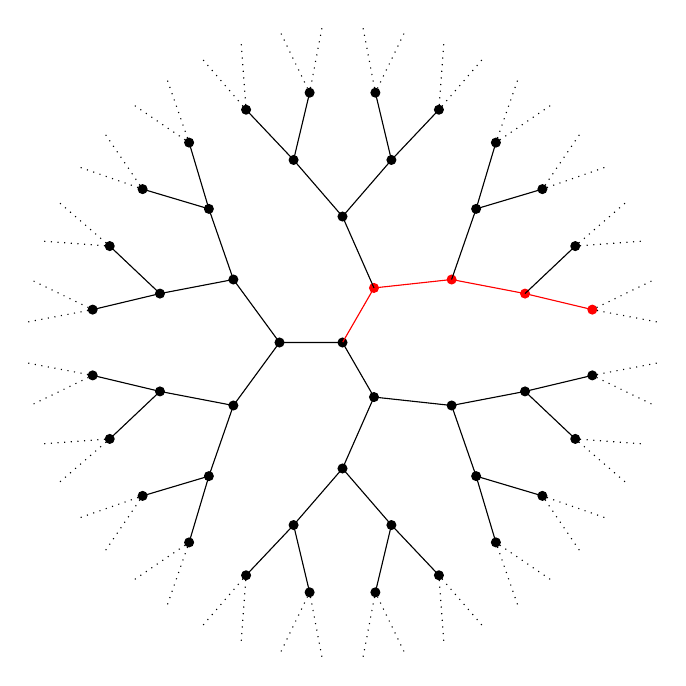
\begin{tikzpicture}[scale=0.8]
        \def\levels{5}
        \draw[fill] (0:0) circle (2pt);
        \foreach \i in {1,...,\levels} {
          \pgfmathparse{3*2^\i}
          \let\nodes\pgfmathresult
          \foreach \j in {1,3,...,\nodes} {
            \pgfmathparse{\j + (-1)^div(\j,2)}
            \let\lower\pgfmathresult
            \uncover<\i->{
              \ifthenelse{\i = \levels}{
                \draw[dotted] (360/\nodes*\j : \i) --
                (360/\nodes*\lower : \i - 1);
              }{
                \pgfextra{
                  \ifthenelse{\j=1}{\def\col{red}}{\def\col{black}}
                  \draw[fill,\col] (360/\nodes*\j : \i) circle (2pt) --
                  (360/\nodes*\lower : \i - 1);
                }
              }
            }
          }
        }
      \end{tikzpicture}
    \end{column}
  \end{columns}
\end{frame}

%%

\begin{frame}
  \centering
  \movie[width=13.5cm,height=7.875cm,loop,poster,autostart,borderwidth=0pt]{}{PathFinding.mp4}
\end{frame}

%%

\begin{frame}{The \textit{smooth} criminals}
  \Large
  \begin{columns}
    \begin{column}{0.7\textwidth}
      \begin{description}
        \setlength{\itemsep}{1em}
      \item[2006] Charles-Goren-Lauter hash function
      \item[2006] Couveignes-Rostovtsev-Stolbunov key exchange
      \item[2011] SIDH key exchange
      \item[2018] CSIDH key exchange
      \end{description}
    \end{column}
    \begin{column}{0.3\textwidth}
      \includegraphics[height=0.8\textheight]{smooth-criminal}
    \end{column}
  \end{columns}
\end{frame}

%%

\begin{frame}{Groups of isogenies}
  \large
  \centering
  \begin{tikzpicture}
    \node (E1) at (0,0) {$B$};
    \node (E) at (6,0) {$A$};

    \draw[-latex] (E) edge[bend right] node[above] {$φ$} (E1)
    edge[bend left] node[above] {$ψ$} (E1);
    \node at (3,-2) {$φ,ψ ∈ \Hom(A,B)$};

    \uncover<2->{
      \draw[-latex] (E) edge node[above] {$φ+ψ$} (E1);
    }

    \uncover<3->{
      \draw[-latex] (E) edge[loop,out=45,in=-45,looseness=10] node[right] {$ω$} (E);
      \node at (8,-2) {$ω ∈ \Hom(A,A)$};
    }
  \end{tikzpicture}

  \uncover<2->{
    \[(φ+ψ)(P) := φ(P) + ψ(P)\]
  }
\end{frame}

%%

\begin{frame}{Endomorphism rings}
  \large
  \begin{itemize}
    \setlength{\itemsep}{2em}
  \item $\Hom(A,B)$ is a group
  \item Distributivity:
    \begin{align*}
      φ∘(ψ+χ) &= (φ∘ψ)+(φ∘χ)\\[2em]
      (ψ+χ)∘φ &= (ψ∘φ)+(χ∘φ)\\
    \end{align*}
  \item It follows that \emph{$\End(A) := \Hom(A,A)$} is a ring.
  \end{itemize}  
\end{frame}

%%

\begin{frame}{Endomorphism rings}
  \large $\End(E)$ is a free $ℤ$-module of rank \textcolor{blue}{1},
  \textcolor{purple}{2} or \textcolor{red}{4}. As a ring:

  \bigskip
  \begin{enumerate}
    \setlength{\itemsep}{1em}
  \item[\color{blue}1)] $\End(E) ≃ ℤ$;
  \item[\color{purple}2)] $\End(E) ⊂$ quadratic imaginary field;
  \item[\color{red}4)] $\End(E) ⊂$ quaternion algebra.
  \end{enumerate}
\end{frame}

%%

\begin{frame}{Isogenies = Ideals}
  \large\centering
  \begin{tikzpicture}
    \node (E1) at (0,0) {$E'$};
    \node (E) at (6,0) {$E$};

    \draw[-latex] (E) edge node[above] {$φ$} (E1);
    \uncover<1>{
      \node at (3,-3) {$φ ∈ \Hom(E,E')$};
    }

    \uncover<2>{
      \draw[-latex] (E) edge[loop,out=45,in=-45,looseness=10] node[right] {$ω$} (E);
      \node at (3,-3) {$φ∘ω ∈ \Hom(E,E')$};
    }
    
    \uncover<3>{
      \draw[-latex] (E1) edge[loop,out=135,in=225,looseness=10] node[left] {$ω'$} (E1);
      \node at (3,-3) {$ω'∘φ ∈ \Hom(E,E')$};
    }
  \end{tikzpicture}
\end{frame}

%%

\begin{frame}{Smoothifying ideals}
  \large
  \begin{columns}
    \begin{column}{0.6\textwidth}
      \centering
      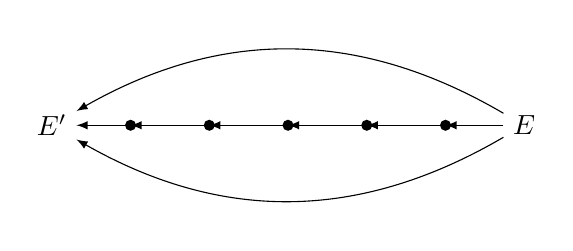
\begin{tikzpicture}
        \node (E1) at (0,0) {$E'$};
        \node (E) at (6,0) {$E$};

        \draw[-latex] (E) edge[bend right] (E1)
        (E) edge[bend left] (E1);
        \uncover<2->{
          \fill[-latex] (E) edge (5,0) (1,0) edge (E1) circle (2pt);
          \foreach \i in {2,...,5} {
            \fill[-latex] (\i,0) edge +(-1,0) circle (2pt);
          }
        }
      \end{tikzpicture}

      \[\Hom(E,E') = \Zφ_1 + \Zφ_2\]

      \uncover<2->{
        \[\deg(\emph{a}φ_1 + \emph{b}φ_2) = \text{\it smooth}\]
      }
    \end{column}
    \begin{column}{0.4\textwidth}
      \centering
      \includegraphics[height=0.8\textheight]{smoothie}
    \end{column}
  \end{columns}
\end{frame}

%%

\begin{frame}{Smoothifying in quadratic imaginary rings}
  \large
  \begin{description}
    \setlength{\itemsep}{1em}
  \item[Algorithm:] Index calculus
  \item[Cost:] exponential complexity, fast in practice
  \item[Used in:] CSI-FiSh signature scheme (2019)
  \end{description}
\end{frame}

%%

\begin{frame}{Smoothifying in quaternion rings}
  \large
  \begin{description}
    \setlength{\itemsep}{1em}
  \item[Algorithm:] Kohel--Petit--Tignol--Lauter (KLPT)
  \item[Cost:] polynomial time
  \item[Used in:] Galbraith--Petit--Silva (2016) and SQIsign (2020)
    signatures
  \end{description}
\end{frame}

%%

\begin{frame}{Basically every isogeny signature}
  \large
  \centering
  \begin{tikzpicture}
    \fill
    (0,0) node(A){} circle (2pt)
    (3,2) node(B){} circle (2pt)
    (6,2) node(C){} circle (2pt)
    (9,0) node(D){} circle (2pt);

    \draw[-latex] (A) edge node[sloped,above] {random} (B)
    (B) edge node[above] {secret key} (C)
    (C) edge node[sloped,above] {random} (D);

    \begin{uncoverenv}<2->
      \foreach \i in {0,...,8} {
        \fill[-latex] (\i,0) edge (\i+1,0) circle (2pt);
      }
      \node at (4.5,-.5) {signature};
    \end{uncoverenv}
  \end{tikzpicture}
\end{frame}

%%

\begin{frame}{SQIsign}
  \begin{table}[h]
    \centering
    \begin{tabular}{ r r r | r r r | c }
      \multicolumn{3}{c|}{Bytes} & \multicolumn{3}{c|}{Mcycles}\\
      Secret Key & Public Key & Signature & Keygen & Sign & Verify & Security \\
      \hline
      782 & 64 & 177 & 3,728 & 5,779 & 108 & NIST-1 \\
      1,138 & 96 & 263 & 23,734 & 43,760 & 654 & NIST-3 \\
      1,509 & 128 & 335 & 91,049 & 158,544 & 2,177 & NIST-5 \\
    \end{tabular}
  \end{table}
\end{frame}

%%

\begin{frame}{What does it mean to ``compute'' an isogeny?}
  \large
  \begin{definition}[Isogeny representation]
    A \textit{representation} of an isogeny \emph{$φ:E→E'$} is an
    \emph{algorithm / Turing machine / arithmetic circuit} that:
    \begin{itemize}
    \item on input \emph{$P ∈ E$}
    \item outputs \emph{$φ(P) ∈ E'$}
    \end{itemize}
    in time polynomial in $\log(\deg φ)$.
  \end{definition}
\end{frame}

%%

\begin{frame}{Higher dimensional abelian varieties}
  \centering
  \begin{tikzpicture}[domain=-2.4566:4,samples=100]
    \begin{scope}[xscale=0.3,yscale=0.5]
      \draw plot (\x,{sqrt(\x*\x*\x-4*\x+5)});
      \draw plot (\x,{-sqrt(\x*\x*\x-4*\x+5)});
      \node (P1) at (3,4.47213595499958) {};
    \end{scope}
    \begin{uncoverenv}<2->
      \begin{scope}[xscale=0.7,yscale=0.15,shift={(7,-20)}]
        \draw plot ({sqrt(\x*\x*\x-4*\x+5)},\x);
        \draw plot ({-sqrt(\x*\x*\x-4*\x+5)},\x);
        \node (P2) at (-4.47213595499958,3) {};
      \end{scope}
      \node at (5,0) {\huge $E×E$};
      
      \fill (P1) circle (2pt);
      \fill (P2) circle (2pt);

      \draw[dashed] (P2) -- (P2 |-, |- P1) -- (P1);
      \fill (P2 |-, |- P1) circle (2pt) node[above right] {$(P,Q)$};
    \end{uncoverenv}
  \end{tikzpicture}
\end{frame}

%%

\begin{frame}{Higher dimensional isogenies}
  \large
  \begin{columns}
    \begin{column}{0.4\textwidth}
      \centering
      \begin{tikzpicture}[scale=2]
        \node (A) at (-1,1) {$A$};
        \node (B) at (1,-1) {$B$};
        \node (C) at (1,1) {$C$};
        \node (D) at (-1,-1) {$D$};

        \draw[-latex] (A) edge node[above] {$α$} (C) edge node[left] {$β$} (D)
        (B) edge node[right] {$γ$} (C) edge node[below] {$δ$} (D);
      \end{tikzpicture}
    \end{column}
    \begin{column}{0.6\textwidth}
      \uncover<2->{
        \begin{align*}
          A × B &→ C × D\\
          (P,Q) &↦ \bigl( α(P) + γ(Q), β(P) + δ(Q) \bigr)\\
                &\uncover<3->{=
                  \begin{pmatrix}
                    α&γ\\β&δ
                  \end{pmatrix}
                  \begin{pmatrix}
                    P\\Q
                  \end{pmatrix}}
        \end{align*}
      }
    \end{column}
  \end{columns}
\end{frame}

%%

\begin{frame}{Kani's lemma}
  \large
  \begin{columns}
    \begin{column}{0.4\textwidth}
      \centering
      \begin{tikzpicture}[scale=2]
        \node (A) at (-1,1) {$A$};
        \node (B) at (1,-1) {$B$};
        \node (C) at (1,1) {$C$};
        \node (D) at (-1,-1) {$D$};

        \draw[-latex] (A) edge node[above] {$α$} (C) edge node[left] {$β$} (D)
        (C) edge node[right] {$γ$} (B)
        (D) edge node[below] {$δ$} (B);

        \node at (0,0) {\Huge $\circlearrowleft$};
      \end{tikzpicture}
    \end{column}
    \begin{column}{0.5\textwidth}
      Let $\deg α = \deg δ$ and $\deg β = \deg γ$ coprime.  The
      isogeny defined by
      \begin{align*}
        Φ : A×B &→ C×D\\
        \begin{pmatrix}
          P\\Q
        \end{pmatrix}
            &↦
                \begin{pmatrix}
                  α & \tilde{γ}\\
                  -β & \tilde{δ}
                \end{pmatrix}
                \begin{pmatrix}
                  P\\Q
                \end{pmatrix}
      \end{align*}      
      is a \emph{$\bigl(\deg(α) + \deg(β)\bigl)$-isogeny} if and only
      if the diagram commutes.

      \bigskip
      
      \uncover<2->{
        \emph{Note:} $Φ(P,0) = \bigl( α(P), -β(P) \bigr)$.
      }
    \end{column}
  \end{columns}
\end{frame}

%%

\begin{frame}{Application: breaking SIDH}
  \large
  \begin{columns}
    \begin{column}{0.4\textwidth}
      \centering
      \begin{tikzpicture}[scale=2]
        \node (A) at (-1,1) {$A$};
        \node (C) at (1,1) {$C$};

        \draw[-latex] (A) edge node[above] {$α$} (C);

        \uncover<2->{
          \node (D) at (-1,-1) {$D$};
          \draw[-latex] (A) edge node[left] {$β$} (D);
        }
        
        \uncover<3->{
          \node (B) at (1,-1) {$B$};
          \draw[latex-] (B) edge (C) edge (D);
          \node at (0,0) {\Huge $\circlearrowleft$};
        }
      \end{tikzpicture}
    \end{column}
    \begin{column}{0.6\textwidth}
      \begin{description}
      \item[Secret:] $α:A→B$ of degree $\deg(α) = d$
      \item[Input:] $α(P)$ for all $P$ of order $2^n > d$
      \item[Goal:] Compute a representation of $α$
      \item[Attack (sketch):]\
        \begin{enumerate}
        \item<2-> Compute an isogeny $β$ of degree \emph{$e = 2^n - d$};
        \item<3-> Complete the commutative square;
        \item<4-> Compute Kani's $2^n$-isogeny $Φ$;
        \item<5-> Then $Φ(P',0) = \bigl(α(P'), \dots\bigr)$ for any $P'∈A$;
        \item<6-> Deduce kernel of $α$;
        \item<7-> Claim 50 K\$.
        \end{enumerate}
      \end{description}
    \end{column}    
  \end{columns}
\end{frame}

%%

\begin{frame}{Application: from quaternions to random isogenies (QFESTA)}
  \large
  \begin{columns}
    \begin{column}{0.4\textwidth}
      \centering
      \begin{tikzpicture}[scale=2]
        \node (A) at (-1,1) {$A$};
        \node (B) at (1,-1) {$A$};
        \node (C) at (1,1) {$C$};
        \node (D) at (-1,-1) {$D$};

        \draw[-latex] (A) edge node[above] {$α$} (C) edge (D)
        (C) edge node[right] {$γ$} (B)
        (D) edge (B);

        \node at (0,0) {\Huge $\circlearrowleft$};
      \end{tikzpicture}
    \end{column}
    \begin{column}{0.6\textwidth}
      \begin{description}
      \item[Input:] $\End(A)$, a degree $d$,
      \item[Output:] A random $d$-isogeny $A→?$.
      \end{description}
      \begin{enumerate}
      \item Find endomorphism $ω$ of degree
        \emph{$\deg ω = d(2^n - d)$},
      \item Factor \emph{$ω = α∘γ$} with \emph{$\deg(α) = d$},
      \item Kani's isogeny is a representation of $α$.
      \end{enumerate}
    \end{column}  
  \end{columns}
\end{frame}

%%

\begin{frame}{Application: evaluate (almost) any ideal (Clapoti)}
  \large
  \begin{columns}
    \begin{column}{0.4\textwidth}
      \centering
      \begin{tikzpicture}[scale=2]
        \node (A) at (0,1) {$A$};
        \node (B) at (1,0) {$A$};
        \node (C) at (1,1) {$C$};
        \draw[-latex] (A) edge node[above]{$d_1$} (C)
        (C) edge node[right]{$d_2$} (B);

        \uncover<2->{
          \node (Au) at (-1,1) {$A_u$};
          \node (Av) at (1,-1) {$A_v$};
          \draw[-latex] (Au) edge node[above]{$u$} (A)
          (B) edge node[right]{$v$} (Av);
        }
        
        \uncover<3->{
          \node (D) at (-1,-1) {$D$};
          \draw[-latex] (Au) edge (D) (D) edge (Av);
        }

        \node at (0,0) {\Huge $\circlearrowleft$};
      \end{tikzpicture}
    \end{column}
    \begin{column}{0.6\textwidth}
      \begin{description}
      \item[Input:] $\End(A)$, an ideal of $\End(A)$,
      \item[Output:] The corresponding isogeny.
      \end{description}
      \begin{enumerate}
      \item Find random equivalent ideals of coprime degrees
        \emph{$d_1,d_2$};
      \item<2-> Find integers $u,v$ s.t. \emph{$ud_1 + vd_2 = 2^n$};
      \item<2-> Find random $u$- and $v$-isogeny;
      \item<3-> Construct Kani square.
      \end{enumerate}
    \end{column}  
  \end{columns}  
\end{frame}

%%

\begin{frame}{Putting it all together: SQIsign2D-West}
  \begin{table}[h]
    \centering
    \begin{tabular}{ r r | r r r | c }
      \multicolumn{2}{c|}{Bytes} & \multicolumn{3}{c|}{Mcycles}\\
      Public Key & Signature & Keygen & Sign & Verify & Security \\
      \hline
      66 & 148 & 60 & 160 & 9 & NIST-1 \\
      98 & 222 & 170 & 460 & 29 & NIST-3 \\
      130 & 294 & 360 & 940 & 62 & NIST-5 \\
    \end{tabular}
  \end{table}
\end{frame}

%%

\begin{frame}[plain]
  \centering
  \begin{tikzpicture}[remember picture,overlay]
    \begin{scope}[xscale=1.7,yshift=-15,opacity=0.8]
      \def\crater{12}
      \def\jumpa{-8}
      \def\jumpb{9}
      \def\diam{5cm}

      \foreach \i in {1,...,\crater} {
        \draw[blue] (360/\crater*\i : \diam) to[bend right] (360/\crater*\i+360/\crater : \diam);
        \draw[red] (360/\crater*\i : \diam) to[bend right] (360/\crater*\i+\jumpa*360/\crater : \diam);
        \draw[green] (360/\crater*\i : \diam) to[bend right=50] (360/\crater*\i+\jumpb*360/\crater : \diam);
      }
    \end{scope}
    
    
    \draw (0,0.5) node{\Huge\bf Thank you};
    \draw (0,-0.6) node{\large\url{https://defeo.lu/}};
    \draw (0,-1.3) node{\large\includegraphics[height=0.9em]{mastodon.png}~\href{https://twitter.com/luca_defeo}{@luca\_defeo@ioc.exchange}};
    \draw (0,-1.9) node{\large
\includegraphics[height=0.9em]{twitter.png}~\href{https://twitter.com/luca_defeo}{@luca\_defeo}};
  \end{tikzpicture}
\end{frame}

\end{document}


% LocalWords:  Isogeny abelian isogenies hyperelliptic supersingular Frobenius
% LocalWords:  isogenous
